% =============================================================================
%
%                             Theory
%
% =============================================================================
% -----------------------------------------------------------------------------
\chapter{Theoretical Background} \label{chapt:theoreticalback}
% -----------------------------------------------------------------------------
This chapter provides the basics of the project. On the one hand, it is about image processing and filtering as well as communication via Ethernet. What kind of image operations are possible and the Wallis filter are explained in the chapter \ref{chapt:theory:imageprocessing}. An overview of the communication via Ethernet is in the chapter \ref{chapt:theory:ethernet}.


% =============================================================================
%
%                          Image Processing
%
% =============================================================================
\section{Image Processing} \label{chapt:theory:imageprocessing}
In technical terms, image processing is the processing of image data. This includes image processing, image analysis and the output of image files \cite{image_processing}. Procedures that generate a new image can be distinguished into point operations, neighborhood operations and global operations based on their input data. \\
The second part explains the Wallis filter used in this project.

% -----------------------------------------------------------------------------
\subsection{Operations}
% -----------------------------------------------------------------------------
The types of operations that can be applied to images to transform an input image I(u, v) to an output image I'(u, v) can be divided into three categories, which are explained in the following three sections.

\subsubsection*{Point Operations}
The point operations use the color or intensity information at a given pixel in the image as input, calculates a new intensity value as the result and stores it to the same point in the target image (figure \ref{fig:image_operation}a). Typical applications of point operations are, for example, the correction of contrast and brightness, color correction by rotating the color space or the application of different threshold value methods.

Example for a point operation with $u$ and $v$ being pixel coordinates:
\begin{equation}
    I'(u, v) = f(I(u, v))
    \label{eq:point_operation}
\end{equation}


\subsubsection*{Neighborhood Operations}
Neighborhood operations use a certain amount of neighboring pixels as input (figure \ref{fig:image_operation}b).
They calculate the result and stored it at the reference point in the target
image. Neighborhood operations are often used in convolution filters. These
filters can be used, for instance, to implement smoothing filters such as the
Gauss filter. Convolution filters can also be used to detect edges in an image. For example, this is possible with the Sobel filter.

Example to calculate the x-derivative and y-derivative with the Sobel matrix \cite{sobel_matrix}:

\noindent\begin{minipage}{.5\linewidth}
\begin{equation}
    G_{x} = I * \begin{bmatrix}
                -1 & 0 & 1 \\ 
                -2 & 0 & 2 \\ 
                -1 & 0 & 1
                \end{bmatrix}
    \label{eq:neighborhood_operation}
\end{equation}

\end{minipage}%
\begin{minipage}{.5\linewidth}

\begin{equation}
    G_{y} = I * \begin{bmatrix}
                -1 & -2 & -1 \\ 
                0 & 0 & 0 \\ 
                1 & 2 & 1
                \end{bmatrix}
    \label{eq:neighborhood_operation}
\end{equation} 

\end{minipage}\\


\textbf{Border Handling:}
With the application of filters, the so-called border handling problem occurs in every image (see figure \ref{fig:image_handling}). Because the filter protrudes beyond the original image.

There are several possible solutions to this issue:
\begin{itemize}
\item The border pixels are not considered. In the example image, the original image 
is two pixels smaller in height and width than the original image. \ref{fig:image_handling}
\item If the filter exceeds the original image, the filter coefficients
at the outside of the image are set to zero
\item The pixels required outside the image are extrapolated according to the closest pixels
\item The image is continued periodically
\end{itemize}
    
\begin{figure}[b!]
    \centering
    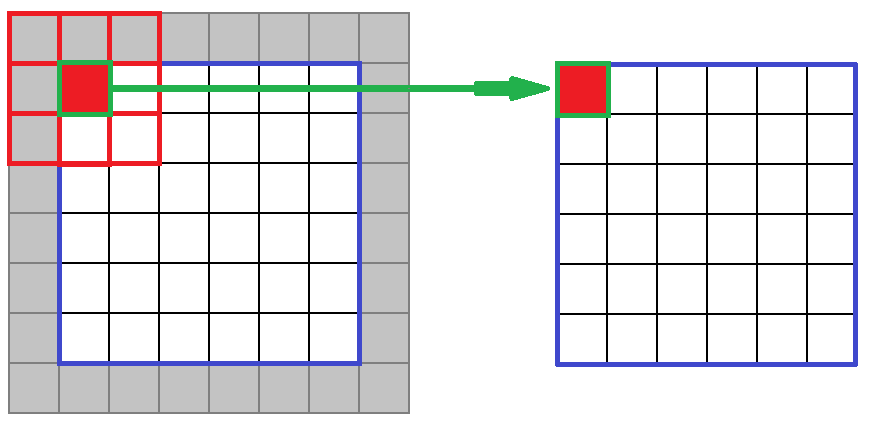
\includegraphics[width=0.6\textwidth]{images/theory/border_handling.png}
    \caption{Border problem with filter operations \cite{border_handling}}
    \label{fig:image_handling}
\end{figure}


\subsubsection*{Global Operations}
Image analysis often employs global image operations that uses the entire image as input data (figure \ref{fig:image_operation}c). It is often about finding regions or recognizing geometrical objects. A typical representative of this is the Hough transform and the Fourier transform.

\begin{figure}[tb!]
    \centering
    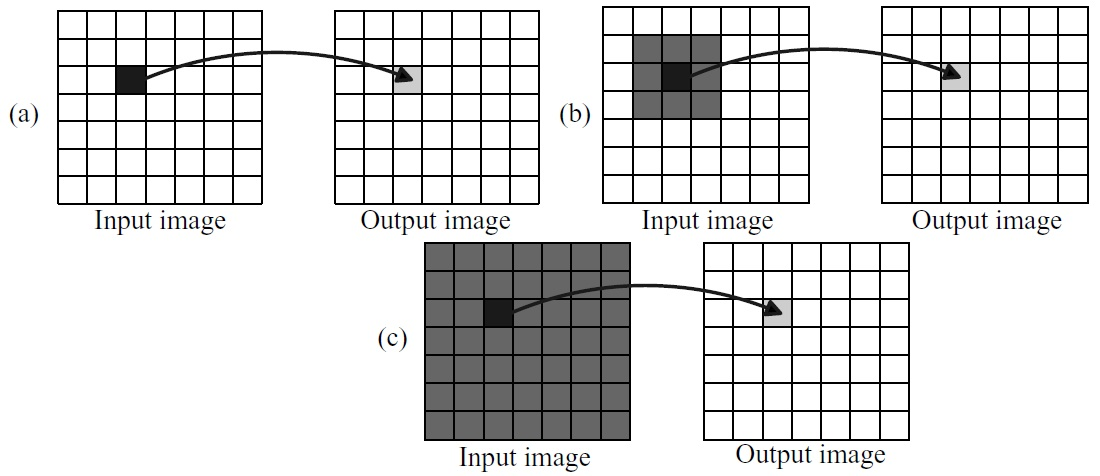
\includegraphics[width=\textwidth]{images/theory/image_operations.jpg}
    \caption{(a) point, (b) neighborhood and (c) global image processing
    operations \cite{image_operation}}
    \label{fig:image_operation}
\end{figure}

% -----------------------------------------------------------------------------
\subsection{Wallis Filter}\label{ch:th_wallis_filter}
% -----------------------------------------------------------------------------
The main goal of the Wallis filter is to adjust the mean and variance of an image and to map it into a given mean and variance to the destination image. This is mainly used for local contrast enhancement in both low and high level regions. It also achieves similair brightness levels in the image.
The Wallis filter equation is \cite{wallis_filter}:
\begin{equation}
    I'(x,y) = \frac{( I(x,y) - \mu_{n})\cdot c \cdot \sigma_{g}^{2}}{c \cdot \sigma_{n}^{2} + (1 - c) \cdot \sigma_{g}^{2}} + b \cdot \mu_{g} + (1 - b) \cdot \mu_{n}
    \label{eq:wallis_filter}
\end{equation} 

\begin{tabular}{rl}
    $I(x,y)         =$ & gray value pixel of the original image \\
    $I'(x,y)        =$ & calculated pixel with the Wallis algorithm \\
    $\mu_{n}        =$ & mean from the neighborhood of the pixel I(x,y) \\
    $\sigma_{n}^{2} =$ & variance from the neighborhood of the pixel I(x,y) \\
    $\mu_{g}        =$ & mean from the destination image \\
    $\sigma_{g}^{2} =$ & variance from the destination image \\
    $b              =$ & brightness factor \\
    $c              =$ & contrast factor \\
\end{tabular} \\

The two facotrs b and c can have the range from 0 to 1. The larger b is selected, the closer it converges to the mean of the desired image $\mu_{g}$. The smaller b is selected, the more it converges to the neighborhood mean $\mu_{n}$.
The bigger the factor c is chosen, the larger is the range of the variance constant $\sigma_{g}^{2}$ \cite{wallis_filter}. \\
The size of the neighborhood depends on the sensor resolution of the camera. The size can be selected from a minimum of 11 to 41 \cite{zeng_2018}. Through the neighborhood operation the smoothing operator is introduced. This means it reduces noise and improves the singal to noise ratio of the image. This in turn enhances image quality \cite{wallis_filter}.


% =============================================================================
%
%                             Ethernet
%
% =============================================================================
\section{Ethernet Communication} \label{chapt:theory:ethernet}
Exchanging data between two devices can be done using different approaches. The
following section contains an overview of the communication standards used in
local area networks (LAN).


\subsection{Open Systems Interconnection (OSI) Model}
Such a telecommunication system can be characterized by the Open Systems 
Interconnection Model. The OSI model is a stack of seven abstraction layers 
grouped into two groups: The host layers and the media layers (see figure \ref{fig:osi}). 
Each layer serves the layer above it and is served with data from the layer
beneath it. In the following chapters the OSI reference model is used to
characterize the Ethernet standard.

\begin{figure}[tb!]
    \centering
    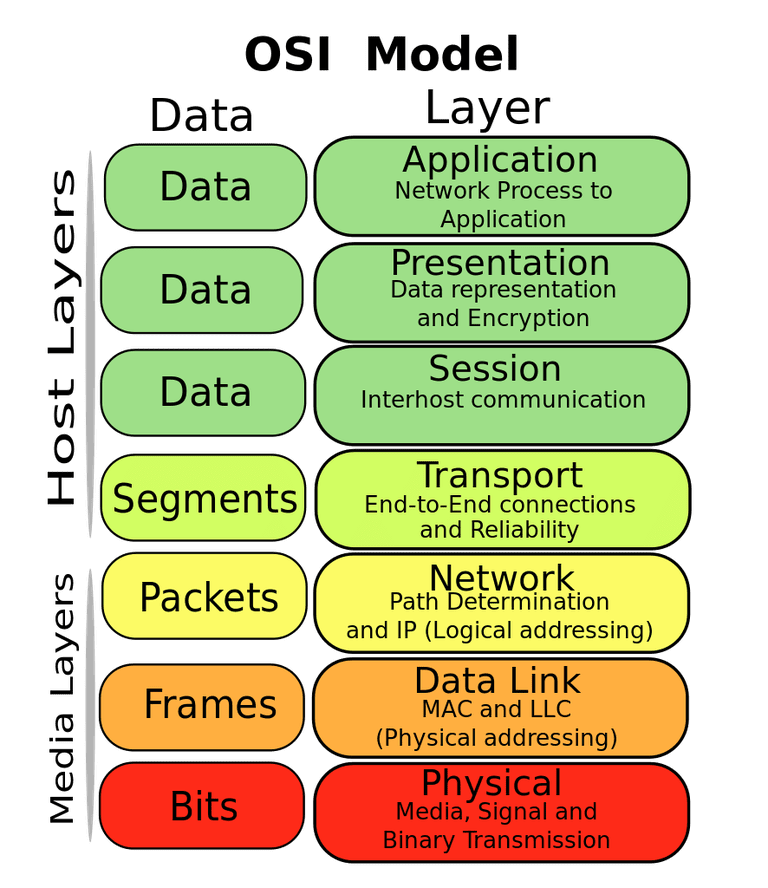
\includegraphics[width=0.5\textwidth]{images/theory/osi.png}
    \caption{OSI Model \cite{osi}}
    \label{fig:osi}
\end{figure}


\subsection{Physical} \label{chapt:theory:physical}
The first layer of the OSI model is the physical layer. It defines the electrical and physical specification of the connection. In the case of local
area networks the connection medium is usually copper. The circuitry required to implement the physical layer is done by the PHY-Chip. This integrated circuit provides digital access through a media independent interface (MII) to the analog physical data link.


\subsection{Data Link} 
The data served from the physical layer is then passed to the data link layer.
Its main purpose is to ensure a reliable transfer of data frames between two
nodes connected by a physical layer. It may also provide means to detect errors
that may occur in the physical layer. Ethernet is the protocol used in the data
layer of local area networks and the layer is split into two sublayers, the logical link control (LLC) and the medium access control (MAC). The LLC provides means to allow multiple network protocols (OSI layer three) to be multiplexed onto the same medium. The MAC encapsulates higher level frames into frames appropriate to be transmitted by the physical layer.
\\

Figure \ref{fig:eth} shows an Ethernet frame. The first seven bytes consist of a fixed preamble. It allows devices on the network to easily synchronize their 
clocks for bit-level synchronization. It is followed by the start frame delimiter (SFD) that marks the beginning of a frame. Sender and receiver MAC addresses ensure that the packet is received by the corresponding host and that it can reply to the sender. The type field indicates the protocol used on the next layer (network layer). After the data payload a frame check sequence in form of a CRC (cyclic redundancy check) is sent to provide error detection. The maximum data payload size is limited to 1500 bytes.
\\

\begin{figure}[tb!]
    \centering
    \begin{adjustbox}{max width=\textwidth}
        \begin{tikzpicture}[
    rounded corners=0mm,
]
    %nodes
    \node[draw, minimum height=1.0cm] (pre) {Preamble};
    \node[draw, minimum height=1.0cm, right = 0cm of pre] (sfd) {SFD};
    \node[draw, minimum height=1.0cm, right = 0cm of sfd] (dst) {Destination MAC Adr.};
    \node[draw, minimum height=1.0cm, right = 0cm of dst] (src) {Source MAC Adr.};
    \node[draw, align = center, text width=1cm, minimum height=1.0cm, right = 0cm of src] (tp) {Type\\Field};
    \node[draw, minimum height=1.0cm, right = 0cm of tp] (dat) {Data (46 - 1500 Bytes)};
    \node[draw, minimum height=1.0cm, right = 0cm of dat] (pad) {PAD};
    \node[draw, minimum height=1.0cm, right = 0cm of pad] (crc) {CRC};

    \path[draw,-] ($(dst.180) + (0,0)$) -- ++(0,1.2) ;
    \path[draw,-] ($(crc.0) + (0,0)$) -- ++(0,1.2) ;
    \path[draw,{Latex[length=2.5mm]}-{Latex[length=2.5mm]}] ($(dst.180) + (0,1.0)$) -- ($(crc.0) + (0,1.0)$) node [midway, above] () {Basic MAC Frame} ;
\end{tikzpicture}
    \end{adjustbox}
    \caption{Ethernet Frame}
    \label{fig:eth}
\end{figure}
The medium access controller is implemented in hardware to ensure that every bit is received and stored. The transmit and receive data is commonly stored in
FiFo (first in first out) buffers. This way the next layer in the OSI model is
not required to have low latency capability.


\subsection{Network} 
The data link layer provides means to send frames across nodes in the same
network. As soon as the destination node is in another network, a network layer
is required. Using logical device addresses, network packets can be routed
across different networks and on different media. This allows data to be sent
over long distances.
\\

The most commonly used network layer is the Internet Protocol version 4 (IPv4).
It consists of a 20 byte sized header that contains destination and source IP
addresses, total length, checksum and other fields. The protocol field indicates what layer four protocol is used. Figure \ref{fig:ip} shows a complete IPv4 header.

\begin{figure}[tb!]
    \centering
    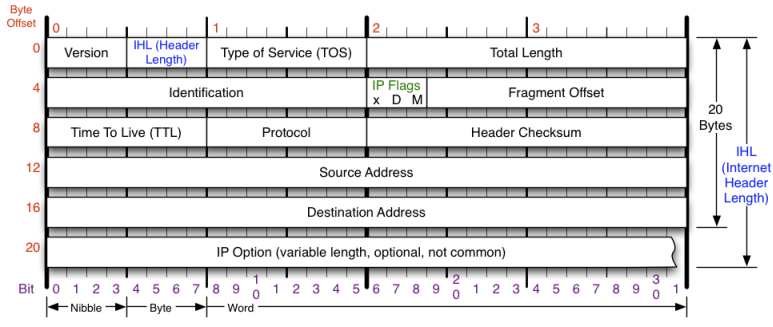
\includegraphics[width=\textwidth]{images/theory/ip.png}
    \caption{IPv4 header \cite{ip}}
    \label{fig:ip}
\end{figure}
\begin{figure}[tb!]
    \centering
    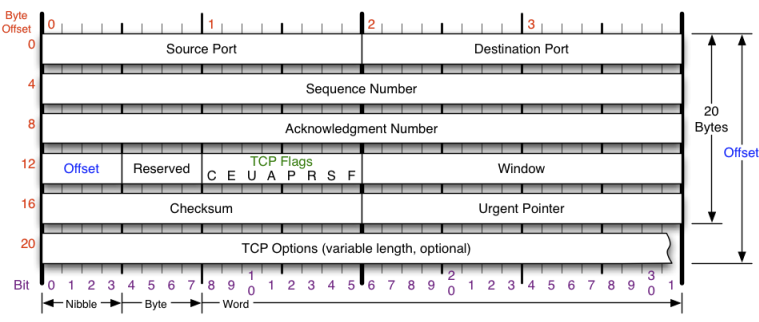
\includegraphics[width=\textwidth]{images/theory/tcp.png}
    \caption{TCP Header \cite{tcpudp}}
    \label{fig:tcp}
\end{figure}
\begin{figure}[tb!]
    \centering
    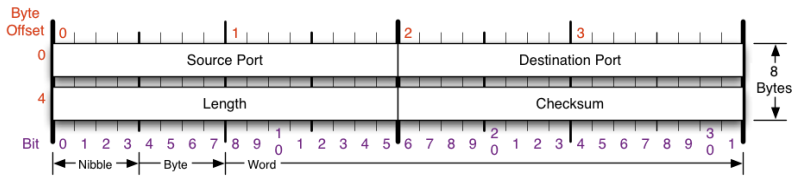
\includegraphics[width=\textwidth]{images/theory/udp.png}
    \caption{UDP Header \cite{tcpudp}}
    \label{fig:udp}
\end{figure}


\subsection{Transport} 
The transport layer is the first layer in the OSI model that is not required by
the network. Its main purpose is to control the communication of different
applications on two hosts. Therefore a port number is required to distinguish
between the different applications utilizing the same network connection. The
transport layer may also provide segmentation of the data, guarantee of delivery and flow control to avoid network jam.
\\

The two most used transport layer protocols are the Transmission Control
Protocol (TCP) and the User Datagram Protocol (UDP). Table \ref{tab:tcpudp}
shows the main differences between these two protocols. The most important
aspect is the protocol connection setup. While UDP is connection less (data is
sent without setup), TCP establishes a connection between host and client
prior to data transmission. This ensures a reliable data delivery hence all
messages are acknowledged. UDP has its benefits in lower overhead and for that
reason has slightly higher transmission speed but the protocol does not
guarantee that the message has been received by the client.

\begin{table}[h]
    \centering
    \begin{tabular}{ l  c  c }
        \toprule
         & \textbf{TCP} & \textbf{UDP} \\
        \midrule
        Connection oriented & Yes & No \\
        Header size & 20 Byte & 8 Byte \\
        Reliable transmission & Yes & No \\
        Acknowledge & Yes & No \\
        Segmentation & Yes & No \\
        Best for & reliable transfer & fast transfer  \\
        \bottomrule
    \end{tabular}
    \caption{TCP vs. UDP}
    \label{tab:tcpudp}
\end{table}
